\section{Selection Operator and Absence in the Standard Sector}
\label{sec:selection}

The effective coupling to the substrate can be written schematically as
\begin{equation}
\mathcal{L}_{\mathrm{int}}
\;\supset\;
\frac{\varepsilon}{\LamUV^{4}}\,
O_S[\phi](x)\,
O_S[\phi](x')\,
\mathcal{K}_{\mathrm{eff}}(x,x'),
\tag{5.1}
\end{equation}
where $O_S$ is a \textbf{pattern complexity operator}. It is designed so that:
\begin{enumerate}
  \item $O_S$ is local, gauge- and diffeomorphism-invariant in $M$;
  \item it is sensitive to \emph{mesoscopic, structured} configurations but strongly suppressed in homogeneous or thermal states;
  \item the combination in Eq.~(5.1) has engineering dimension four so that $\varepsilon$ is dimensionless.
\end{enumerate}

\subsection{Seed operator and dimensionality}
\label{sec:selection:seed}

Start from a local, gauge-invariant ``seed'' operator $\mathcal{O}(x)$ built from visible fields and curvature, with mass dimension
$\Delta>4$ (irrelevant in the Wilsonian sense). We then define a
\emph{normalized} operator
\begin{equation}
  O_S(x)
  :=
  \frac{\mathcal{O}(x)}{\Lambda^{\Delta-4}},
  \qquad
  [O_S]=4,
  \quad
  [\varepsilon]=0.
  \tag{5.2}
\end{equation}
Here $\Lambda$ is a fixed UV scale of the visible sector. Choosing $\Delta>4$ makes $\mathcal{O}$ irrelevant in the Wilsonian sense, which provides technical naturalness for a small coupling. However, \emph{we do not rely on RG running to hide the effect from colliders}. The key point is that renormalizing to $[O_S]=4$ removes the energy-dependence from the operator itself; all dimensional analysis is done at the Lagrangian level with fixed $\LamUV$. What \emph{actually} suppresses visible-sector signatures is the state-dependence of $\langle O_S\rangle$ via degeneracy dilution, as explained next. In what follows we only use that $O_S$ is local, gauge- and diffeomorphism-invariant, built from irrelevant operators with $\Delta>4$, and normalized to $[O_S]=4$; its detailed field content is otherwise unconstrained.

\subsection{Degeneracy dilution in homogeneous states}

For homogeneous, periodic, or thermal configurations (collider beams, crystals, near-equilibrium baths), there are $N \gg 1$ macroscopically equivalent realizations (embeddings) of any given local pattern inside a large volume. We design the selection operator $O_S$ so that it "rewards" a specific embedding (or a finite set of embeddings) of the pattern.

In a translation-invariant or high-entropy state that has no preference for any specific embedding, the coarse-grained state is effectively a mixture or random superposition over all $N$ possibilities. As shown in the toy model of Appendix I, the probability weight for the specific embedding singled out by $O_S$ scales inversely with the volume:

\begin{equation}
|\langle O_S \rangle_{hom}| \sim \frac{O_0}{N} \implies \mathcal{Q} \sim \frac{1}{N} \to 0 \quad (N \to \infty)
\end{equation}

This is the precise sense in which the pattern signal is "diluted": the overlap with the specific pattern targeted by $O_S$ shrinks as $1/N$. Thus:

\begin{equation}
\langle O_S \rangle_{thermal/periodic} \approx 0, \quad \langle O_S \rangle_{structured} = \mathcal{O}(1)
\end{equation}

Consequently, the aether-resonance channel is effectively switched off in ordinary homogeneous matter, including collider beams and cosmological fluids.

\begin{figure}[h]
\centering
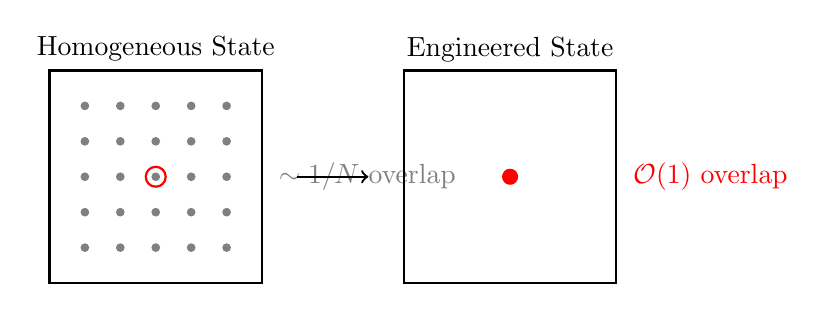
\begin{tikzpicture}[scale=0.9]
  % Left: Homogeneous
  \draw[thick] (0,0) rectangle (3,3);
  \node at (1.5, 3.3) {Homogeneous State};
  \foreach \x in {0.5, 1.0, ..., 2.5}
    \foreach \y in {0.5, 1.0, ..., 2.5}
      \filldraw[gray] (\x,\y) circle (1.5pt);
  \draw[red, thick] (1.5, 1.5) circle (4pt); % Target
  \node[right, gray] at (3.1, 1.5) {$\sim 1/N$ overlap};

  % Right: Engineered
  \draw[thick] (5,0) rectangle (8,3);
  \node at (6.5, 3.3) {Engineered State};
  \filldraw[red] (6.5, 1.5) circle (3pt); % Target
  \node[right, red] at (8.1, 1.5) {$\mathcal{O}(1)$ overlap};
  
  % Arrow
  \draw[->, thick] (3.5, 1.5) -- (4.5, 1.5);
\end{tikzpicture}
\caption{Degeneracy dilution. Left: In a homogeneous state, the selection operator $O_S$ (red circle) has small overlap with the $N$ equivalent embeddings. Right: In an engineered state, the pattern is pinned, yielding macroscopic overlap.}
\label{fig:dilution}
\end{figure}

\subsection{Structured states and pattern quality}
\label{sec:selection:structured}

In contrast, in a driven, mesoscopic, pattern-rich system (engineered materials, critical networks, biological tissues, etc.) the pattern encoded by $O_S$
can be realized in only a few places, and its overlap with the actual state can approach unity. We summarize this as
\begin{equation}
  \langle O_S\rangle \;\propto\; \mathcal{Q}\,\tilde{\Delta\Phi},
  \qquad
  0 \le \mathcal{Q} \le 1,
  \tag{5.5}
\end{equation}
where:
\begin{itemize}
  \item $\mathcal{Q}$ is a dimensionless \emph{pattern quality factor} (introduced more explicitly in Sec.~6), which measures how well the configuration matches the targeted pattern;
  \item $\tilde{\Delta\Phi}$ is a dimensionless free-energy difference associated with driving the system between two nearby macrostates in $S$.
\end{itemize}
The dependence on the structural distance $d_\sigma$ resides in the kernel $\Ksig = \exp[-d_\sigma/\lambda_\sigma]$ (Sec.~7). For large structural separations, $\Ksig\to 0$ and the coupling vanishes even if $\mathcal{Q}$ is high.

\subsection{Explicit example of a local $O_S$}

One convenient class of examples is based on a windowed functional of derivatives and curvature. Let $w_\ell(x)$ be a smooth, compactly supported window of linear size $\ell$, and define
\begin{equation}
  O_S(x)
  =
  \frac{1}{\Lambda^{\Delta-4}}
  \int d^4y\,\sqrt{-g(y)}\,
  w_\ell(x-y)\,
  \mathcal{F}\!\big(
    \nabla\phi(y),\,
    \nabla\nabla\phi(y),\,
    R_{\mu\nu\rho\sigma}(y)
  \big),
  \tag{5.6}
\end{equation}
with
\begin{equation}
  \mathcal{F}
  :=
  \sum_{m+n+k=\Delta} c_{mnk}\,
  \big(\nabla\phi\big)^{m}\,
  \big(\nabla\nabla\phi\big)^{n}\,
  \big(R_{\mu\nu\rho\sigma}\big)^{k},
  \tag{5.7}
\end{equation}
and coefficients $c_{mnk}$ chosen so that $O_S$ is scalar, gauge-invariant, and UV-soft above its design scale. The window function ensures locality on scales $\lesssim \ell$, while the polynomial structure makes $O_S$ sensitive to higher-order patterns (gradients, curvature, correlations) rather than just local field amplitudes.

Two genericity remarks are important here.  First, for a ``generic''
choice of coefficients $c_{mnk}$ (e.g.\ drawn from a broad, symmetric
distribution subject only to gauge invariance and UV softness), the
operator $O_S$ is highly sensitive to mesoscopic pattern structure but
its expectation value in homogeneous, periodic, or thermal states is
suppressed by degeneracy dilution.  If there are $N\gg 1$ macroscopically
equivalent ways of placing a given pattern inside such a state, then a
typical superposition of those placements yields
$\langle O_S\rangle \sim N^{-1/2}$ or smaller.  In the thermodynamic
limit this drives the quality factor $Q$ to zero.

Second, moving away from homogeneous states does not require fine
tuning of $c_{mnk}$.  Instead, one engineers platforms (Sec.~5.3) in
which the patterns singled out by $O_S$ are realized in only a few
locations with correlated phases (for example, near critical points or
edge-of-chaos regimes in complex networks).  In such states the overlap
with $O_S$ can approach order unity, $Q\sim 1$, while keeping the same
underlying definition of $O_S$.  In this sense the selection operator
is generic at the level of its field content; what is special is the
prepared state of the visible sector. All later constraints on the S-channel depend only on these generic properties of $O_S$---locality, symmetry, and degeneracy dilution---rather than on the particular choice of window function $w_\ell$ or polynomial $F$ in Eq.~(5.6).

\subsection{Why colliders see nothing}

Putting the pieces together, the effective contribution of Eq.~(5.1) to any collider observable schematically scales as
\begin{equation}
  \mathcal{A}_{\mathrm{collider}}
  \;\sim\;
  \varepsilon\,
  \langle O_S\rangle_{\mathrm{in}}\,
  \langle O_S\rangle_{\mathrm{out}}\,
  K_{\sigma,\mathrm{eff}},
  \tag{5.8}
\end{equation}
where ``in'' and ``out'' denote initial and final states in a high-energy experiment. For realistic beams and final states we expect:
\begin{itemize}
  \item approximate translational and rotational invariance;
  \item rapidly decorrelating phases;
  \item large degeneracy $N$ of equivalent pattern placements.
\end{itemize}
By the degeneracy-dilution argument (spelled out explicitly in the toy
model of Appendix~\ref{app:degeneracy-toy-model}), $\langle O_S\rangle_{\mathrm{in}}\approx
\langle O_S\rangle_{\mathrm{out}}\approx 0$ in such states, so that collider
cross-sections are suppressed by the \emph{state} rather than by RG
running. The same logic applies to cosmological and astrophysical plasmas that are nearly homogeneous on microscopic scales.

In summary, the selection operator $O_S$ is chosen so that:
\begin{itemize}
  \item it is technically natural and irrelevant in the Wilsonian sense (built from operators with $\Delta>4$ and normalized as in Eq.~(5.2));
  \item it has negligible expectation value in homogeneous, periodic, or thermal states due to degeneracy dilution;
  \item it can attain order-one values only in specially engineered, near-critical, pattern-rich systems, which are precisely the regimes targeted by our proposed experiments in Sec.~13.
\end{itemize}

\subsection{Radiative Stability via Pattern Sequestering}

A generic bilinear coupling between the visible sector and a Lorentz-violating substrate would typically induce dangerous lower-dimension operators (e.g., SME coefficients $\kappa_{JK}$) via vacuum loops. In standard EFT, these would be suppressed only by the coupling $\varepsilon$, leading to potential conflict with experimental bounds of order $10^{-18}$.

To resolve this, we introduce the \textbf{Pattern Sequestering Assumption}: the S-channel is not a universal modification of the vacuum, but a conditional channel active only in the presence of complex order.

We formalize this by treating the pattern-activation field $Q_*(x)$ introduced in Eq.~(3.1) as a background spurion. The interaction Lagrangian scales as:

\begin{equation}
\mathcal{L}_{int} \propto \varepsilon \, Q_*^2(x) \, O_S \, \chi
\end{equation}

This structure imposes specific constraints on radiative corrections:

\begin{enumerate}
\item \textbf{Vacuum Sequestering:} In the vacuum, homogeneous fluids, or standard collider environments used to define SME bounds, the pattern activation is negligible ($Q_* \equiv 0$). Consequently, the S-sector decouples entirely in these regimes. No S-induced Lorentz-violating operators are generated in the effective action for standard model fields in the vacuum background.

\item \textbf{Pattern Parity:} The $Q_*^2$ dependence is consistent with a discrete "Pattern Parity" symmetry ($Z_2^P$), under which $Q_* \to -Q_*$, $\chi \to -\chi$, and $O_S \to -O_S$, while visible fields remain even. This symmetry forbids all radiative corrections odd in the spurion, preventing linear leakage of Lorentz violation into the vacuum sector.

\item \textbf{Active Regime:} In the engineered systems targeted by experiments E1-E3, the spurion acquires a non-zero value $Q_* \sim \mathcal{Q}$, activating the channel. Radiative corrections in this regime are proportional to $\varepsilon Q^2$, which remains consistent with the phenomenological bounds discussed in Sec.~11.
\end{enumerate}

\emph{Loop-level scaling and SME coefficients.}---In a standard Wilsonian treatment, the interaction
\[
\mathcal{L}_{\rm int} \supset \varepsilon\,Q_*^2\,O_S\,\chi
\]
generates loop diagrams with two insertions of $\mathcal{L}_{\rm int}$ connected by $\chi$ and visible-field propagators. Schematically, a dimension-4 Lorentz-violating operator $\mathcal{O}_{\rm LV}$ in the visible sector (for example a photon-sector tensor contributing to $\tilde\kappa_{e-}$ in SME language) will appear with a coefficient of the form
\[
\delta c_{\rm LV} \sim \frac{(\varepsilon Q_*^2)^2}{16\pi^2}\,f\!\left(\frac{\Lambda}{\mu}\right),
\]
where $\Lambda$ is a UV cutoff for the effective description, $\mu$ is a renormalization scale, and $f$ is a dimensionless loop function of order unity. In homogeneous or vacuum backgrounds we set $Q_*\equiv 0$, so these coefficients vanish identically at any loop order: there is no radiative leakage of Lorentz violation into the vacuum EFT. In an engineered high-$Q$ configuration one has $Q_*\sim Q\ll 1$, so that induced coefficients scale at least as $\varepsilon^2 Q^4$. For benchmark values $\varepsilon\lesssim 10^{-15}$ and ambitious targets $Q\lesssim 10^{-2}$, this places loop-generated photon-sector coefficients safely below the existing bounds discussed in Sec.~11 even if the S-channel comes close to saturating the thermodynamic resource inequality.

A complete multi-loop matching calculation to the full SME parameter set would require specifying a UV completion of the S-sector and is beyond the scope of this work. What we rely on in this paper is the structural statement that every Lorentz-violating operator in the visible-only EFT carries at least two powers of $Q_*$ and therefore vanishes in the homogeneous and vacuum regimes where current SME bounds are obtained.

This sequestering mechanism turns the radiative stability problem into a structural statement about the substrate: the pattern-local channel is strictly conditional on the presence of active pattern complexity.
